\chapter{cstelm}

\section{Introduction}

An LPE may have parameters that do not change value throughout the state space of that process.
These parameters are essentially \emph{constant}.
Removing constant parameters results in a smaller state vector (which may improve performance), but otherwise the state space of an LPE remains the same.

Constants can be safely removed from a process as follows:
\begin{enumerate}
\item Substitute references to a constant parameter by the initial (explicit) value of that parameter;
\item Remove the constant from the process parameter list.
\end{enumerate}

\section{Algorithm}

The algorithm consists of the following steps \cite{groote2001computer}:

\begin{enumerate}

\item Make it so that all LPE parameters are \labeledas{constant}.

\item Let $X$ be the set of all LPE parameters that are \labeledas{constant}.
Define a substitution $V = [p \rightarrow v_I(p) \;|\; p \in X]$, where $v_I(p)$ gives the initial value of LPE parameter $p$.

\item Consider each summand $s$ of the LPE.
Construct an equation $g_s \rightarrow p = v_s(p)$ for all $p \in X$, where $g_s$ is the guard of $s$ and where $v_s(p)$ is the expression that defines the value of LPE parameter $p$ after the application of summand $s$, and apply the substitution $V$ to it.
(This gives $(g_s \rightarrow p = v_s(p))[V] \Leftrightarrow {g_s}[V] \rightarrow v_I(p) = v_s(p)[V]$.)

If the obtained equation is a tautology (that is, if its negation is unsatisfiable) for all $s$, $p$ remains \labeledas{constant}; otherwise, \removelabelfrom{constant} $p$.

\item Repeat the previous two steps until the fixpoint of $X$ is reached.
Then remove all LPE parameters that are still \labeledas{constant} from the LPE, substituting references to those parameters by their initial values.

\end{enumerate}

\section{Example}

Consider the following LPE:

\begin{lstlisting}
//Process definition:
PROCDEF example[A](x, y, z :: Int)
  = A [[z = 2]] >-> example[A](z-1, 1, 2)
  + A >-> example[A](y, x, x+y)
  + A >-> example[A](1, x, z+1)
  ;

//Initialization:
example[A](1, 1, 2);
\end{lstlisting}

First, $V = [ x \rightarrow 1, y \rightarrow 1, z \rightarrow 2 ]$.

We must check the following equations:

\begin{align*}
(z = 2 \rightarrow x = z-1)[V] &\Leftrightarrow (2 = 2 \rightarrow 1 = 2-1) \Leftrightarrow \textit{true} \\
(z = 2 \rightarrow y = 1)[V] &\Leftrightarrow (2 = 2 \rightarrow 1 = 1) \Leftrightarrow \textit{true} \\
(z = 2 \rightarrow z = 2)[V] &\Leftrightarrow (2 = 2 \rightarrow 2 = 2) \Leftrightarrow \textit{true} \\
(x = y)[V] &\Leftrightarrow (1 = 1) \Leftrightarrow \textit{true} \\
(y = x)[V] &\Leftrightarrow (1 = 1) \Leftrightarrow \textit{true} \\
(z = x+y)[V] &\Leftrightarrow (2 = 1+1) \Leftrightarrow \textit{true} \\
(x = 1)[V] &\Leftrightarrow (1 = 1) \Leftrightarrow \textit{true} \\
(y = x)[V] &\Leftrightarrow (1 = 1) \Leftrightarrow \textit{true} \\
(z = z+1)[V] &\Leftrightarrow (2 = 2+1) \Leftrightarrow \textit{false} \\
\end{align*}

The last equation is not a tautology, and the `constant' label is therefore removed from $z$.

The new value of $V$ is $[ x \rightarrow 1, y \rightarrow 1 ]$.

\clearpage
The equations are now the following:

\begin{align*}
(z = 2 \rightarrow x = z-1)[V] &\Leftrightarrow (z = 2 \rightarrow 1 = z-1) \Leftrightarrow \textit{true} \\
(z = 2 \rightarrow y = 1)[V] &\Leftrightarrow (z = 2 \rightarrow 1 = 1) \Leftrightarrow \textit{true} \\
(x = y)[V] &\Leftrightarrow (1 = 1) \Leftrightarrow \textit{true} \\
(y = x)[V] &\Leftrightarrow (1 = 1) \Leftrightarrow \textit{true} \\
(x = 1)[V] &\Leftrightarrow (1 = 1) \Leftrightarrow \textit{true} \\
(y = x)[V] &\Leftrightarrow (1 = 1) \Leftrightarrow \textit{true} \\
\end{align*}

All of the equations above are tautologies, and so $x$ and $y$ remain labeled with `constant'.
A fixpoint has been reached; removing $x$ and $y$ from the LPE gives

\begin{lstlisting}
//Process definition:
PROCDEF example[A](z :: Int)
  = A [[z==2]] >-> example[A](2)
  + A [[true]] >-> example[A](2)
  + A [[true]] >-> example[A](z+1)
  ;

//Initialization:
example[A](2);
\end{lstlisting}

Obviously, more simplification is possible.
Applying the \texttt{clean} command (see \ref{clean}) gives

\begin{lstlisting}
//Process definition:
PROCDEF example[A](z :: Int)
  = A [[true]] >-> example[A](2)
  + A [[true]] >-> example[A](z+1)
  ;

//Initialization:
example[A](2);
\end{lstlisting}

\section{Benchmark results}

The following durations were measured with a benchmark for several models:
\begin{itemize}
\item The average duration of \txs{} to make 500 steps in a model after it has been converted to LPE form;
\item The average duration of \txs{} to make 500 steps in a model after it has been converted to LPE form and after the \texttt{cstelm} operation has been applied.
\end{itemize}

When plotting the second series of measurements against the first (see Figure~\ref{cstelm-vs-lpe-only:fig}), it becomes clear that the effect of \texttt{cstelm} is tiny.

\begin{figure}[!ht]
\begin{center}
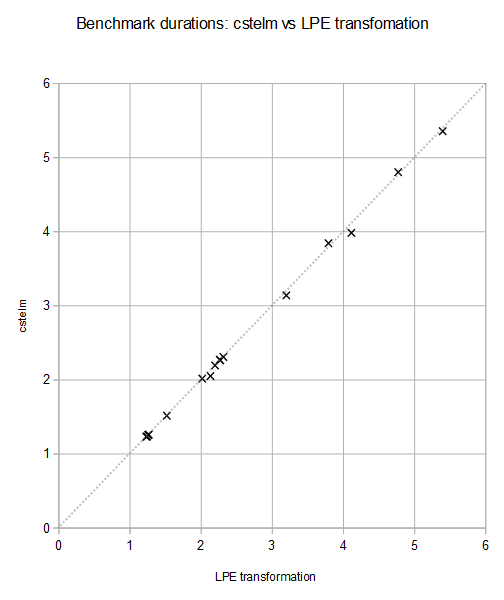
\includegraphics[width=0.7\linewidth]{charts/cstelm-vs-lpe-only}
\caption{Benchmark results: cstelm vs LPE transformation}
\label{cstelm-vs-lpe-only:fig}
\end{center}
\end{figure}

